\documentclass[11pt,a4paper,oneside]{report}
\usepackage[spanish,activeacute,es-noshorthands]{babel}
\usepackage[utf8]{inputenc}
\usepackage[T1]{fontenc}
\usepackage{lmodern}
\usepackage{amsmath, amssymb}
\usepackage{graphicx}
\usepackage[dvipsnames]{xcolor}
\usepackage{geometry}
\geometry{margin=2.4cm, headheight=14pt}
\usepackage{microtype}
\usepackage{booktabs}
\usepackage{enumitem}
\usepackage{fancyhdr}
\usepackage{tcolorbox}
\tcbuselibrary{skins, breakable}
\usepackage{caption}
\captionsetup{font=small, labelfont=bf}
\usepackage{hyperref}
\hypersetup{
  colorlinks=true,
  linkcolor=NavyBlue,
  citecolor=ForestGreen,
  urlcolor=BrickRed,
  pdftitle={Guion --- Experimento de mascaras opticas lensless},
  pdfauthor={INTISAT Payload --- CubeSat-EdgeAI}
}

\graphicspath{{./}{../out/}{../out/previews/}{./Medida/}}

\definecolor{intisat}{RGB}{26, 54, 93}
\definecolor{intisataccent}{RGB}{197, 143, 0}
\definecolor{ok}{RGB}{47, 133, 90}
\definecolor{warn}{RGB}{197, 60, 60}

% Cajas de callout
\newtcolorbox{decir}[1][]{
  colback=blue!4, colframe=intisat,
  fonttitle=\bfseries, title=Lo que decis al presentar,
  breakable, sharp corners=south, #1
}
\newtcolorbox{calculo}[1][]{
  colback=gray!5, colframe=gray!50,
  fonttitle=\bfseries, title=Calculo,
  breakable, sharp corners=south, #1
}
\newtcolorbox{hipotesis}[1][]{
  colback=yellow!8, colframe=intisataccent,
  fonttitle=\bfseries, title=Hipotesis,
  breakable, sharp corners=south, #1
}
\newtcolorbox{riesgo}[1][]{
  colback=red!5, colframe=warn,
  fonttitle=\bfseries, title=Riesgo,
  breakable, sharp corners=south, #1
}
\newtcolorbox{accion}[1][]{
  colback=green!5, colframe=ok,
  fonttitle=\bfseries, title=Accion,
  breakable, sharp corners=south, #1
}

\pagestyle{fancy}
\fancyhf{}
\fancyhead[L]{\nouppercase{\leftmark}}
\fancyhead[R]{\thepage}
\renewcommand{\headrulewidth}{0.4pt}

\title{
  {\Huge\bfseries\color{intisat} Guion del experimento}\\[0.3em]
  {\LARGE Mascaras opticas para microscopia lensless}\\[0.6em]
  {\large Estudio comparativo de rendijas: \textit{circular, cuadrada y lineal}}
}
\author{INTISAT Payload --- \texttt{CubeSat-EdgeAI-Payload}}
\date{\today}

\begin{document}

\begin{titlepage}
\centering
\vspace*{1cm}
{\color{intisat}\rule{\textwidth}{2pt}}
\vspace{0.6cm}

{\Huge\bfseries\color{intisat} Guion del experimento}

\vspace{0.3cm}
{\LARGE\bfseries Mascaras opticas para microscopia lensless}

\vspace{0.6cm}
{\Large\itshape Estudio comparativo de rendijas: circular, cuadrada y lineal}

\vspace{1cm}
{\color{intisataccent}\rule{0.6\textwidth}{1pt}}

\vspace{2.5cm}

\begin{tabular}{rl}
\textbf{Sensor:} & OV5647 (lensless) \\
\textbf{Iluminacion:} & OLED SSD1351 RGB 128$\times$128 \\
\textbf{Plataforma:} & INTISAT --- payload de microscopia FPM \\
\textbf{Repositorio:} & \texttt{github.com/JaminYC/CubeSat-EdgeAI-Payload} \\
\textbf{Fecha:} & \today
\end{tabular}

\vfill

{\large
Este documento es el \textbf{guion completo} del experimento: incluye lo que se dice al
presentar, los calculos opticos, las hipotesis predichas para cada mascara,
el procedimiento paso a paso, las metricas a medir y los resultados esperados.
Acompaña a la presentacion \texttt{Presentacion\_Mascaras\_Lensless.pptx}
y a las imagenes generadas en \texttt{out/}.
}

\vspace{1.2cm}
{\color{intisat}\rule{\textwidth}{2pt}}
\end{titlepage}

\tableofcontents
\clearpage

% =====================================================================
\chapter{Resumen ejecutivo}

\begin{decir}
``Hoy presento un experimento de tres mascaras fisicas que disenamos en CAD para montar
sobre el sensor OV5647 lensless del payload. La pregunta es simple: \textbf{¿que mascara
da el mejor compromiso entre nitidez de imagen y luz disponible para celulas biologicas?}
Vamos a probarlas en tres modos de ensamblaje diferentes (9 combinaciones en total)
y medir 6 metricas cuantitativas sobre cada captura.''
\end{decir}

El experimento responde tres preguntas:

\begin{enumerate}[leftmargin=2.2em]
  \item ¿Cual de las tres geometrias (\emph{rendija}, \emph{cuadrada}, \emph{circular})
        da mejor calidad de imagen para una muestra biologica?
  \item ¿Que diferencias visibles aparecen en cada caso (forma del FOV, contraste,
        artefactos de difraccion)?
  \item ¿En que modo de ensamblaje (A/B/C) cada mascara funciona mejor?
\end{enumerate}

Las decisiones tomadas para mantener el experimento controlado:

\begin{itemize}[leftmargin=2.2em]
  \item Misma muestra en todas las pruebas: epidermis de cebolla (corte $\sim 5\times 5$ mm).
  \item Misma iluminacion: patron \emph{bright-field} uniforme del OLED.
  \item Total de capturas: \textbf{9 condiciones} (idealmente 3 repeticiones cada una $=$ 27).
  \item Tiempo estimado total: 1--2 horas de experimento $+$ 30 min de procesado.
\end{itemize}

% =====================================================================
\chapter{Concepto fisico: por que necesitamos una mascara}

\begin{decir}
``Sin lente, cada punto de la muestra dispersa luz hacia muchos pixeles del sensor
--- eso produce \emph{blur}. Lo unico que tenemos para limitar esa dispersion es una
\textbf{mascara fisica} que restringe los angulos. La pregunta es: \textbf{que forma}
le damos al hueco de esa mascara, y \textbf{donde} la ponemos.''
\end{decir}

\section{Geometria fundamental}

Si la apertura tiene tamaño caracteristico $D$ y esta a distancia $h$ del sensor:
\begin{equation}
\boxed{\;\mathrm{NA} = \sin\!\left(\arctan\!\frac{D}{2h}\right) \approx \frac{D}{2h}\;\;\;\text{(angulos chicos)}}
\label{eq:na}
\end{equation}

\begin{calculo}
La resolucion teorica esta dada por el limite de Abbe:
\[
d_{\min} = \frac{\lambda}{2\,\mathrm{NA}} \quad \text{con}\quad \lambda \approx 550\;\text{nm}
\]
Por ejemplo, para $\mathrm{NA} = 0{,}29 \Rightarrow d_{\min} \approx 0{,}96\;\mu\text{m}$.
Los pixeles del OV5647 son de $1{,}4\;\mu\text{m}$ --- por lo que la NA $\approx 0{,}3$ alcanza para que el
sensor sea el limitante (no la optica).
\end{calculo}

\begin{decir}
``\textbf{Importante:} las dimensiones reales de las mascaras
(medidas sobre el modelo CAD final en Inventor) son
$\varnothing\,3{,}000$ mm para el pinhole, $3{,}054 \times 3{,}054$ mm para la cuadrada
y $0{,}178 \times 5{,}606$ mm para el slit. La profundidad del housing es $h = 5{,}0$ mm.
Esos numeros son los que usamos en todos los calculos.''
\end{decir}

\section{Tabla de NA en funcion de $D$ y $h$}

\begin{center}
\begin{tabular}{cccc}
\toprule
\textbf{$h$ (mm)} & \textbf{Pinhole 3.000 mm} & \textbf{Cuadrada 3.054 mm} & \textbf{Slit 0.178 mm} \\
\midrule
2.0 & 0.60 (37°) & 0.61 (37°) & 0.044 (3°) \\
3.0 & 0.45 (27°) & 0.45 (27°) & 0.030 (2°) \\
\textbf{5.0} (real) & \textbf{0.29 (17°)} & \textbf{0.29 (17°)} & \textbf{0.018 (1°)} \\
7.0 & 0.21 (12°) & 0.22 (12°) & 0.013 (1°) \\
10.0 & 0.15 (9°) & 0.15 (9°) & 0.009 (0.5°) \\
\bottomrule
\end{tabular}
\end{center}

\begin{decir}
``\textbf{Regla a recordar:}
NA bajo $\rightarrow$ nitidez alta pero poca luz.
NA alto $\rightarrow$ mucha luz pero blur. Toda la decision experimental gira en torno a este compromiso.''
\end{decir}

% =====================================================================
\chapter{Las tres mascaras fabricadas}

\begin{decir}
``Disenamos tres placas de $25\times 25$ mm con el mismo contorno exterior y orejas
de fijacion --- la \textbf{unica diferencia} entre ellas es la forma del hueco central.
Eso garantiza que cualquier diferencia que veamos en las imagenes viene exclusivamente
de la geometria de la apertura, no del montaje mecanico.''
\end{decir}

\section{Mascara 1 --- Rendija lineal (slit)}

\begin{figure}[h!]
\centering
\includegraphics[width=0.7\textwidth]{{Muesca Rejilla}.png}
\caption{Mascara con rendija (slit). Vista superior del CAD: 5 ranuras paralelas verticales,
ancho \textbf{$0{,}178$ mm $= 178\;\mu$m}, largo \textbf{$5{,}606$ mm} (medido en Inventor).}
\label{fig:muesca-slit}
\end{figure}

\begin{figure}[h!]
\centering
\includegraphics[width=0.78\textwidth]{{Medida 1 muescarejilla}.png}
\caption{Medicion CAD de la rendija: ancho minimo $0{,}178$ mm.}
\end{figure}

\begin{calculo}
Eje corto (ancho de la rendija): $w = 0{,}178$ mm, con $h = 5{,}0$ mm:
\[
\mathrm{NA}_{\text{corto}} = \frac{0{,}178}{2 \cdot 5{,}0} = 0{,}0178 \quad
\Rightarrow \quad d_{\min} \approx \frac{0{,}55}{2 \cdot 0{,}0178} \approx 15{,}4\;\mu\text{m}
\]
Eje largo: $L = 5{,}606$ mm. La NA en ese eje es alta ($\approx 0{,}49$) y el blur queda libre $\Rightarrow$
imagen tipo \emph{line scan} (cinco bandas paralelas nitidas).
\end{calculo}

\section{Mascara 2 --- Apertura cuadrada}

\begin{figure}[h!]
\centering
\includegraphics[width=0.7\textwidth]{{Muesca Cuadrada}.png}
\caption{Mascara con apertura cuadrada. Lado \textbf{$3{,}054$ mm} (medido en Inventor).}
\label{fig:muesca-cuadrada}
\end{figure}

\begin{figure}[h!]
\centering
\includegraphics[width=0.78\textwidth]{{Medida Muesca cuadrada}.png}
\caption{Medicion CAD de la cuadrada: lado $3{,}054$ mm.}
\end{figure}

\begin{calculo}
Lado $s = 3{,}054$ mm con $h = 5{,}0$ mm:
\[
\mathrm{NA}_{\text{eje}} = \sin(\arctan(s/2h)) = \sin(\arctan(0{,}305)) = 0{,}292,
\]
\[
\mathrm{NA}_{\text{diagonal}} = \sin(\arctan(s\sqrt{2}/2h)) \approx 0{,}396.
\]
Area $= s^2 = 9{,}33$ mm$^2$ (la mas grande de las tres mascaras).
\end{calculo}

\section{Mascara 3 --- Pinhole circular}

\begin{figure}[h!]
\centering
\includegraphics[width=0.7\textwidth]{{Muesca Circular}.png}
\caption{Mascara con pinhole circular. Diametro \textbf{$\varnothing\,3{,}000$ mm} (medido en Inventor).}
\label{fig:muesca-circular}
\end{figure}

\begin{figure}[h!]
\centering
\includegraphics[width=0.78\textwidth]{{Medida Muesca circular}.png}
\caption{Medicion CAD del pinhole: $\varnothing\,3{,}000$ mm, radio $1{,}500$ mm.}
\end{figure}

\begin{calculo}
Diametro $D = 3{,}000$ mm con $h = 5{,}0$ mm:
\[
\mathrm{NA} = \sin(\arctan(D/2h)) = \sin(\arctan(0{,}30)) = 0{,}287
\]
\[
d_{\text{Airy}} = \frac{1{,}22 \cdot 0{,}55}{2 \cdot 0{,}287} \approx 1{,}17\;\mu\text{m}
\]
Area $= \pi (D/2)^2 = 7{,}07$ mm$^2$ ($75\%$ de la cuadrada).
\end{calculo}

\section{Las camaras (housings) que sostienen cada mascara}

Cada mascara va alojada en una \emph{camara} (housing) impresa en negro mate que define
la distancia $h$ al sensor. \textbf{Profundidad efectiva real: $h = 5{,}0$ mm} (medida sobre el modelo CAD).

\begin{figure}[h!]
\centering
\begin{tabular}{ccc}
\includegraphics[width=0.3\textwidth]{{Camara Rejilla}.png} &
\includegraphics[width=0.3\textwidth]{{Camara Cuadrada}.png} &
\includegraphics[width=0.3\textwidth]{{Camara Circular}.png} \\
Camara para slit & Camara para cuadrada & Camara para circular
\end{tabular}
\caption{Housings 3D para cada mascara. Profundidad efectiva $h = 5{,}0$ mm.}
\label{fig:camaras}
\end{figure}

\begin{figure}[h!]
\centering
\includegraphics[width=0.32\textwidth]{{Medida Camara circular}.png}
\hfill
\includegraphics[width=0.32\textwidth]{{Medida 2 Camara cuadrada}.png}
\hfill
\includegraphics[width=0.32\textwidth]{{Medida Camara rectanular rejilla}.png}
\caption{Mediciones CAD de los housings. Cilindrico exterior $\varnothing\,8{,}586$ mm
(circular y cuadrada) o caja $7{,}620$ mm (rejilla). Profundidad mascara--sensor: $5{,}0$ mm.}
\end{figure}

% =====================================================================
\chapter{Tres modos de ensamblaje sobre el OV5647}

\begin{decir}
``La misma mascara puede montarse de tres formas diferentes. Cada modo tiene un
compromiso distinto entre nitidez y control angular. Vamos a probar las 3 mascaras
$\times$ 3 modos $=$ 9 combinaciones para mapear el espacio de soluciones.''
\end{decir}

\begin{figure}[h!]
\centering
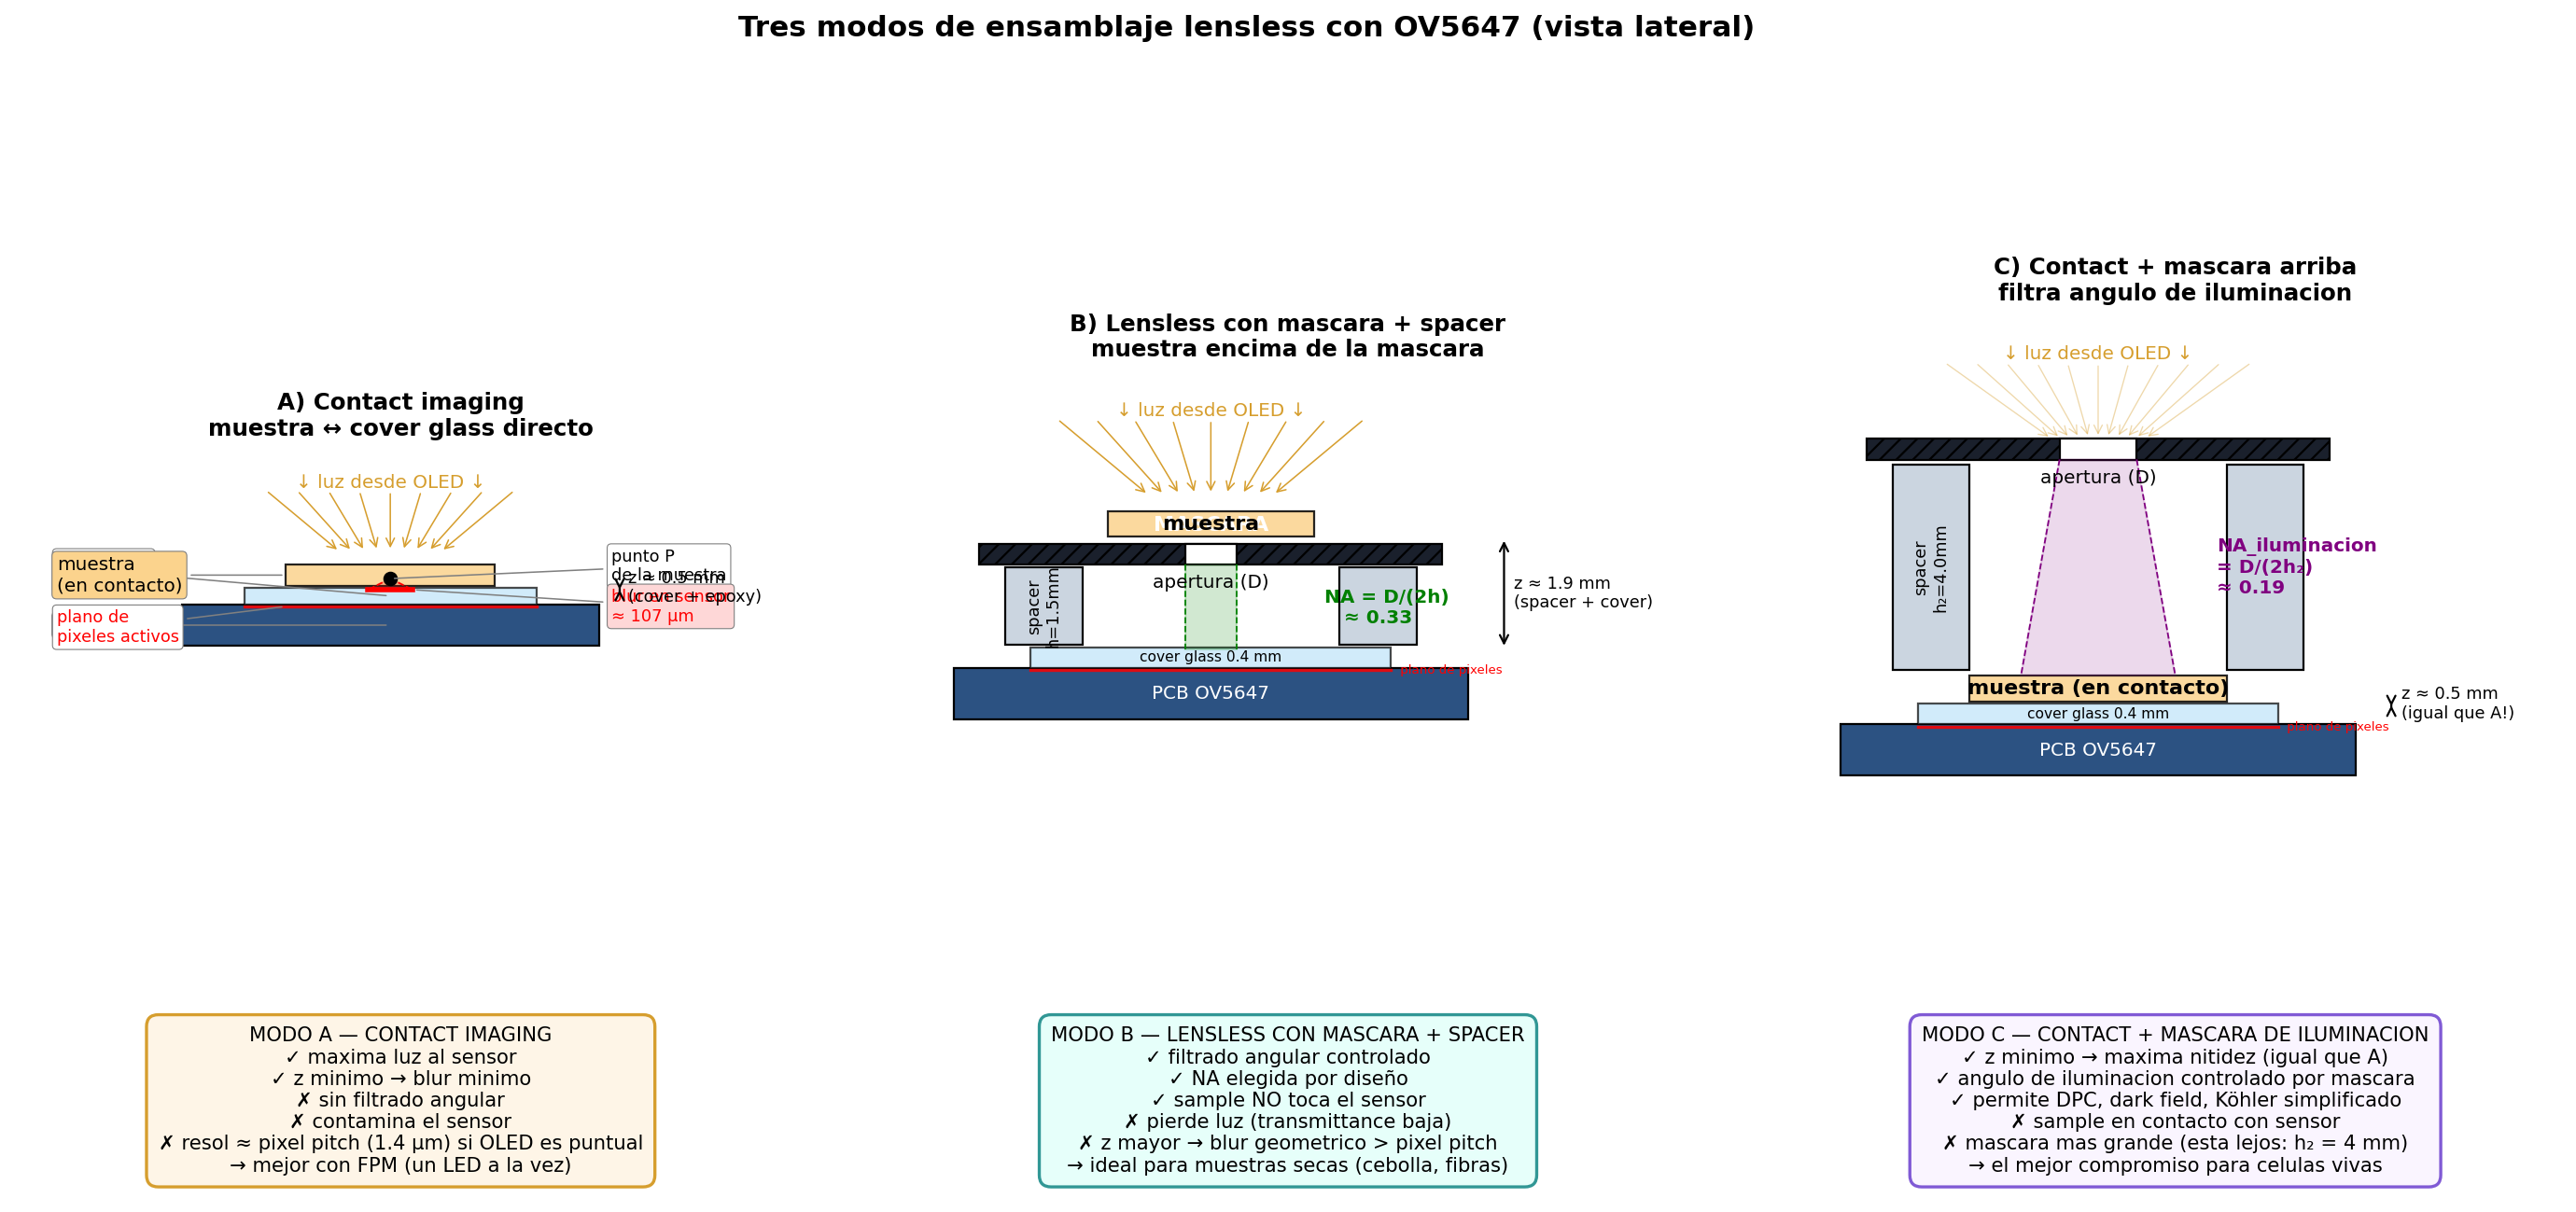
\includegraphics[width=\textwidth]{aperture_masks_assembly.png}
\caption{Comparacion de los tres modos. \textbf{(A)} contact imaging: muestra apoyada en el
cover glass, sin mascara. \textbf{(B)} lensless con mascara y spacer: la mascara va entre
el cover glass y la muestra. \textbf{(C)} contact con mascara arriba: muestra en contacto
y mascara separada para controlar el angulo de \emph{iluminacion}.}
\label{fig:modos}
\end{figure}

\section{Caracteristicas distintivas}

\begin{itemize}[leftmargin=2.2em]
  \item \textbf{Modo A (contact imaging):} maxima luz, $z \approx 0{,}5$ mm. Sin filtrado angular.
        Apto solo si la fuente es \emph{puntual} (FPM con un LED a la vez).
  \item \textbf{Modo B (lensless con mascara y spacer):} filtrado angular del lado de
        \emph{coleccion}. La NA del sensor queda dada por la apertura. Sample no toca el sensor.
  \item \textbf{Modo C (contact + mascara arriba):} mantiene $z = 0{,}5$ mm
        (la nitidez de A) pero agrega control sobre el angulo de \emph{iluminacion}
        que llega a la muestra. Permite DPC, dark field y oblique illumination.
\end{itemize}

% =====================================================================
\chapter{Hipotesis por mascara}

% --- Slit ---
\section{Hipotesis 1 --- Rendija lineal}

\begin{figure}[h!]
\centering
\includegraphics[width=0.4\textwidth]{{Muesca Rejilla}.png}
\hspace{0.5cm}
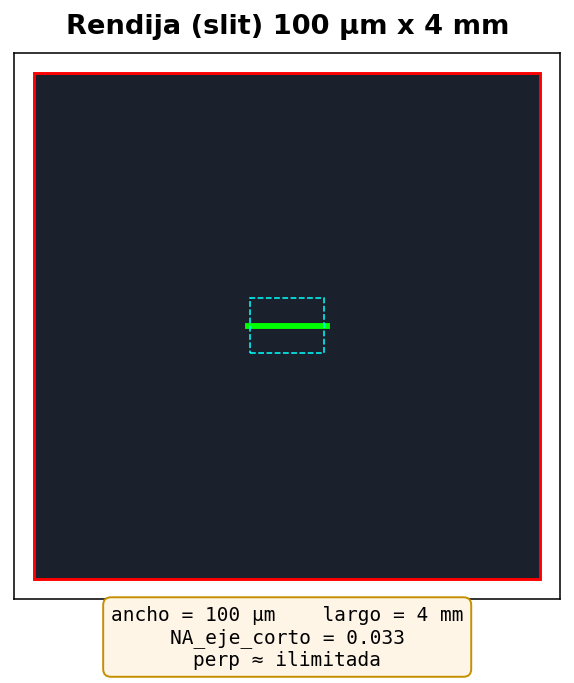
\includegraphics[width=0.4\textwidth]{rendija_(slit)_100_µm_x_4_mm.png}
\caption{Izquierda: CAD de la mascara slit. Derecha: simulacion 2D con su area activa
del sensor proyectada (cuadro discontinuo cyan).}
\end{figure}

\begin{hipotesis}
\begin{itemize}[leftmargin=1.5em]
  \item Resolucion \textbf{baja} ($\sim 15\;\mu$m) en el eje perpendicular a la rendija
        --- significativamente peor que las otras dos.
  \item Resolucion \textbf{alta} en el eje paralelo.
  \item Imagen tipo \emph{multi-line scan}: cinco bandas paralelas nitidas (5 ranuras).
  \item Util para confirmar el plano de enfoque y para perfilometria de paredes celulares.
  \item SNR moderado --- comparable a la cuadrada al sumar las cinco ranuras.
\end{itemize}
\end{hipotesis}

\textbf{Que vamos a ver en la imagen:} una banda horizontal o vertical de unos pocos
cientos de micrometros de ancho, donde las paredes celulares se ven nitidas, y un fondo
borroso a los costados que decae con un perfil aproximadamente $\mathrm{sinc}(\pi w \cdot u)$
donde $w$ es el ancho de la rendija y $u$ la frecuencia espacial.

% --- Cuadrada ---
\section{Hipotesis 2 --- Apertura cuadrada}

\begin{figure}[h!]
\centering
\includegraphics[width=0.4\textwidth]{{Muesca Cuadrada}.png}
\hspace{0.5cm}
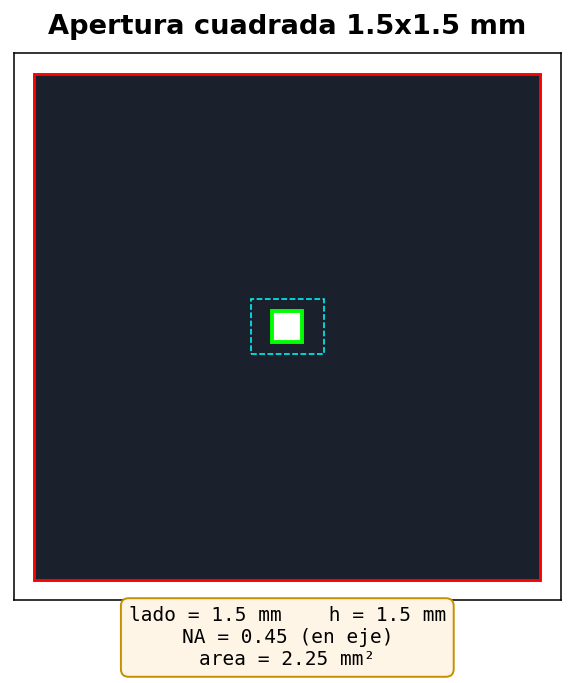
\includegraphics[width=0.4\textwidth]{apertura_cuadrada_1.5x1.5_mm.png}
\caption{Izquierda: CAD de la mascara cuadrada. Derecha: simulacion 2D.}
\end{figure}

\begin{hipotesis}
\begin{itemize}[leftmargin=1.5em]
  \item FOV cuadrado bien definido --- los bordes rectos seran visibles en la imagen.
  \item Resolucion uniforme en X e Y, anisotropica respecto a la diagonal.
  \item \textbf{Mas luz} que el pinhole circular (area $= 9{,}33$ mm$^2$ vs $7{,}07$ mm$^2$, $32\%$ mas).
  \item Difraccion en las esquinas: aparecen patrones cruzados (PSF separable $\mathrm{sinc}^2 \times \mathrm{sinc}^2$).
  \item Bueno para test de calibracion: el cuadrado en la imagen confirma alineacion.
\end{itemize}
\end{hipotesis}

\textbf{Que vamos a ver en la imagen:} un area cuadrada de $\sim 3{,}6\times 2{,}7$ mm
(limitada por el sensor, no por la mascara) con paredes celulares nitidas en el centro
y vignetting suave hacia los bordes. La PSF de difraccion es separable
$\mathrm{sinc}(x)\,\mathrm{sinc}(y)$, asi que cualquier punto brillante intenso va a
mostrar \emph{cruces} caracteristicas alineadas a los ejes.

% --- Circular ---
\section{Hipotesis 3 --- Pinhole circular}

\begin{figure}[h!]
\centering
\includegraphics[width=0.4\textwidth]{{Muesca Circular}.png}
\hspace{0.5cm}
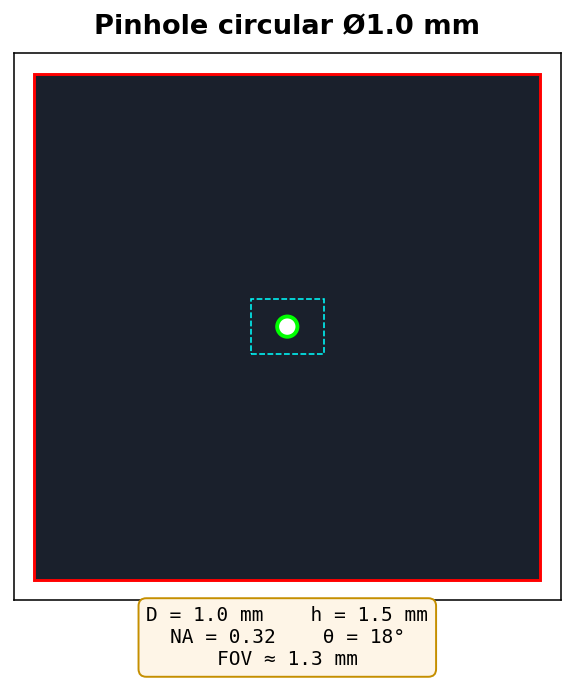
\includegraphics[width=0.4\textwidth]{pinhole_circular_d1.0_mm.png}
\caption{Izquierda: CAD del pinhole circular. Derecha: simulacion 2D.}
\end{figure}

\begin{hipotesis}
\begin{itemize}[leftmargin=1.5em]
  \item FOV circular --- el contorno es un disco uniforme.
  \item Resolucion isotropica $\sim 1\;\mu$m (similar a la cuadrada).
  \item Patron Airy: anillos concentricos cuando hay difraccion intensa.
  \item Es \textbf{el estandar de comparacion} (todos los textos de optica usan pinhole).
  \item Menos area que la cuadrada ($7{,}07$ vs $9{,}33$ mm$^2$) $\Rightarrow$ menos luz, pero PSF mas predecible.
  \item La mas confiable para \textbf{contar celulas} con el pipeline de IA
        --- la PSF Airy es la mas predecible.
\end{itemize}
\end{hipotesis}

\textbf{Que vamos a ver en la imagen:} un disco circular completo dentro del sensor (en B)
o casi todo el sensor cubierto (en A o C, donde la mascara controla otro parametro).
La PSF es un disco de Airy $\propto [J_1(\pi D u)/(\pi D u)]^2$, con primer cero en
$u = 1{,}22\,\lambda/D$.

% =====================================================================
\chapter{Matriz experimental: 3 mascaras $\times$ 3 modos}

\begin{decir}
``Cada celda de esta tabla es un experimento. Misma muestra, misma iluminacion,
unica variable: como armamos el sandwich optico.''
\end{decir}

\begin{center}
\renewcommand{\arraystretch}{1.4}
\begin{tabular}{p{2.6cm}p{3.5cm}p{3.5cm}p{4cm}}
\toprule
\textbf{Mascara $\backslash$ Modo} & \textbf{A) contact} & \textbf{B) lensless $+$ spacer} & \textbf{C) contact $+$ mascara arriba} \\
\midrule
\textbf{Slit (rendija)} &
\textit{shadow line scan $+$ blur OLED} &
\textit{line scan claro, perdida de luz} &
\textit{DPC con corte X o Y} \\
\textbf{Cuadrada} &
\textit{FOV cuadrado borroso} &
\textit{FOV cuadrado nitido $+$ mas luz} &
\textit{iluminacion cuadrada controlada} \\
\textbf{Pinhole} &
\textit{FOV circular borroso} &
\textit{FOV circular nitido --- referencia} &
\textit{Köhler simplificado, contraste limpio} \\
\bottomrule
\end{tabular}
\end{center}

\begin{accion}
\textbf{Plan logistico:}
\begin{itemize}[leftmargin=1.5em]
  \item 9 capturas (idealmente 3 repeticiones por celda $\Rightarrow$ 27 capturas).
  \item Cada captura: 1 imagen RAW $+$ 1 imagen procesada $+$ log JSON.
  \item Tiempo por celda: $\sim 5$ min (incluye montaje, alineacion y captura).
  \item Total experimento: $\sim 1$--2 h.
\end{itemize}
\end{accion}

% =====================================================================
\chapter{Metricas a medir}

\begin{decir}
``Para que el experimento sea cientifico y no \emph{visual}, definimos 6 metricas
cuantitativas. Todas estan ya implementadas en el pipeline; solo hay que correrlo
sobre cada captura.''
\end{decir}

\begin{center}
\renewcommand{\arraystretch}{1.5}
\small
\begin{tabular}{p{2.7cm}p{3.5cm}p{3.5cm}p{3.7cm}}
\toprule
\textbf{Metrica} & \textbf{Definicion} & \textbf{Como se mide} & \textbf{Que esperamos} \\
\midrule
Resolucion (FWHM) &
Ancho a media altura de un borde &
Edge spread function (ESF) sobre una pared celular &
cuadrada $\approx$ pinhole (1 $\mu$m) $<$ slit (15 $\mu$m eje fino) \\
Contraste (Michelson) &
$(I_{\max}{-}I_{\min}) / (I_{\max}{+}I_{\min})$ &
ROI de celula vs fondo &
pinhole $>$ cuadrada $>$ slit \\
SNR &
$\mu / \sigma$ en zona uniforme &
ROI lejos de la muestra &
cuadrada $>$ pinhole $>$ slit \\
FOV utilizable &
\% del sensor con buena nitidez &
Binarizar Laplaciano y contar pixels &
cuadrada $>$ pinhole $>$ slit \\
\# celulas detectadas &
Salida del segmentador StarDist &
Pipeline automatico &
cuadrada (mas luz $+$ FOV) o pinhole \\
Brillo medio &
Valor de gris promedio &
Media de la ROI muestra &
cuadrada $>$ pinhole $>$ slit \\
\bottomrule
\end{tabular}
\end{center}

\begin{decir}
``Las predicciones de la ultima columna son hipotesis. Si el experimento las confirma,
sabremos que entendemos el sistema. Si las contradice, hay algo que no modelamos
y aprendemos algo nuevo --- las dos opciones son utiles.''
\end{decir}

% =====================================================================
\chapter{Cuadro de resultados esperados}

Sintesis cualitativa de las hipotesis. Las estrellas indican rendimiento esperado:
$\star\star\star =$ excelente, $\star\star =$ bueno, $\star =$ marginal.

\begin{center}
\renewcommand{\arraystretch}{1.5}
\begin{tabular}{p{4cm}ccc}
\toprule
 & \textbf{Slit (rendija)} & \textbf{Cuadrada} & \textbf{Pinhole circular} \\
\midrule
Resolucion (eje fino)     & $\star$               & $\star\star\star$       & $\star\star\star$  \\
Resolucion uniforme       & ---                   & $\star\star\star$       & $\star\star\star$  \\
Luz / SNR                 & $\star\star$          & $\star\star\star$       & $\star\star$       \\
FOV                       & $\star$ (linea)       & $\star\star\star$       & $\star\star$       \\
Simplicidad de analisis   & $\star\star$          & $\star\star$            & $\star\star\star$  \\
Caso de uso preferido     & line-scan, perfilometria & lensless general & calibracion, referencia \\
\bottomrule
\end{tabular}
\end{center}

\begin{accion}
\textbf{Recomendacion preliminar (a confirmar con el experimento):}
\begin{itemize}[leftmargin=1.5em]
  \item \textbf{Pinhole circular} $=$ referencia metrologica (la prediccion mas confiable, PSF Airy bien estudiada).
  \item \textbf{Cuadrada} $=$ workhorse para uso general (mas luz, FOV completo del sensor).
  \item \textbf{Slit} $=$ caso especial; util para line-scanning o medir un eje con maxima resolucion.
\end{itemize}
\end{accion}

% =====================================================================
\chapter{Procedimiento experimental}

\begin{decir}
``Esta es la receta paso a paso. La idea es que cualquier persona del equipo pueda
reproducir el experimento sin pedirme aclaraciones. Si te trabas en algun paso,
documentalo --- esa es la parte mas valiosa del experimento.''
\end{decir}

\section{Paso 0 --- Calibracion previa}

\begin{enumerate}[leftmargin=2.2em]
  \item Imprimir / cortar las 3 mascaras (PLA negro 0.4 mm o aluminio anodizado).
  \item Verificar dimensiones reales con calibre o microscopio comparando contra
        los valores CAD: $\varnothing\,3{,}000$ pinhole, $3{,}054$ cuadrada,
        $0{,}178 \times 5{,}606$ rejilla. Anotar discrepancias en
        \texttt{exp\_<fecha>/calibration.json}.
  \item Verificar la altura del housing $h = 5{,}0$ mm con calibre.
  \item Capturar imagen de la regleta de 1 mm en cada modo (A, B, C) para obtener el
        $\mu$m/pixel real (no asumir $2{,}66$). Anotar en el log.
\end{enumerate}

\section{Paso 1 --- Preparacion}

\begin{enumerate}[leftmargin=2.2em]
  \item Limpiar el cover glass del OV5647 con isopropilico y un paño de microfibra.
  \item Preparar la muestra: corte de epidermis de cebolla $\sim 5\times 5$ mm,
        deshidratado entre dos coverslips de vidrio.
  \item Verificar el OLED: encender en patron \emph{full white} (todos los pixeles
        encendidos) y confirmar uniformidad visual.
\end{enumerate}

\section{Paso 2 --- Captura por celda}

Para \textbf{cada} combinacion mascara $\times$ modo:

\begin{enumerate}[leftmargin=2.2em]
  \item Montar la mascara con su housing (\emph{camara}) correspondiente.
        Verificar la distancia $h$ con calibre.
  \item Encender el OLED en patron uniforme (bright-field).
  \item Disparar 3 capturas consecutivas via
        \texttt{python -m cubesat.daemon --capture --tag exp\_<mask>\_<mode>}.
  \item Visualmente, confirmar que la imagen no este saturada
        (histograma centrado, sin clipping).
  \item Si esta saturada: bajar el tiempo de exposicion. Si esta oscura: subirlo.
        Anotar el tiempo final en el log.
\end{enumerate}

\section{Paso 3 --- Procesamiento}

\begin{enumerate}[leftmargin=2.2em]
  \item Correr el pipeline completo:
        \texttt{python -m pipeline.controller run --input exp\_<fecha>/}.
  \item El pipeline genera, por cada captura:
        \texttt{overlay.png}, \texttt{mask.png}, \texttt{data.csv},
        \texttt{summary.json} con todas las metricas del Capitulo 6.
  \item Consolidar todas las \texttt{summary.json} en una tabla pivot por mascara/modo.
\end{enumerate}

\section{Paso 4 --- Analisis y conclusiones}

\begin{enumerate}[leftmargin=2.2em]
  \item Por cada metrica, generar un boxplot (3 mascaras $\times$ 3 modos).
  \item Confirmar/refutar cada hipotesis del Capitulo 5.
  \item Identificar las celdas con resultados \emph{inesperados} y ahondar en ellas.
  \item Escribir \texttt{exp\_<fecha>/RESULTS.md} con conclusiones, sorpresas y
        proximos pasos.
  \item Subir todo a GitHub bajo \texttt{experiments/<fecha>\_mascaras/}.
\end{enumerate}

% =====================================================================
\chapter{Riesgos y proximos pasos}

\section{Riesgos identificados}

\begin{riesgo}
\begin{itemize}[leftmargin=1.5em]
  \item \textbf{Tolerancias de fabricacion:} si la rendija de $178\;\mu$m sale a $250\;\mu$m,
        la NA cambia $\times 1{,}4$ y las predicciones se corren.
        \emph{Mitigacion}: medir cada mascara con microscopio antes del experimento.
  \item \textbf{Profundidad del housing:} $h$ esta en $5{,}0$ mm por diseño, pero la
        impresion 3D puede tener error $\pm 0{,}1$ mm $\Rightarrow$ NA $\pm 2\%$.
  \item \textbf{Alineacion mecanica:} descentrado de $0{,}5$ mm $=$ sombra del borde de la mascara
        cae sobre el sensor.
        \emph{Mitigacion}: usar las orejas con tornillos M2 y verificar simetria visualmente.
  \item \textbf{Iluminacion no uniforme:} el OLED puede tener gradiente $\Rightarrow$ afecta el
        contraste medido. \emph{Mitigacion}: capturar tambien una imagen \emph{flat-field}
        sin muestra para correccion post-hoc.
  \item \textbf{Reflexiones internas:} el lado expuesto al sensor debe ser \textbf{mate}
        (negro PLA o anodizado). Brillante $\Rightarrow$ ghosts cruzados.
  \item \textbf{Limpieza:} una mota en la mascara aparece como punto oscuro fijo en
        \emph{todas} las capturas $\Rightarrow$ falsos positivos en deteccion.
        \emph{Mitigacion}: limpieza con aire comprimido + verificacion previa.
\end{itemize}
\end{riesgo}

\section{Proximos pasos}

\begin{accion}
Una vez completado este experimento basico:

\begin{enumerate}[leftmargin=2.2em]
  \item Repetir las 9 capturas con OLED en \emph{single-LED} (una posicion a la vez)
        para ver cuanto cambia el blur con iluminacion puntual.
  \item Probar la mascara \textbf{honeycomb} ($5\times 5$ pinholes) como cuarto candidato:
        ¿da mejor compromiso entre luz y nitidez?
  \item Implementar DPC: 4 capturas con la mascara C en cuatro orientaciones
        (left/right/top/bottom). Reconstruir el mapa de fase $\Rightarrow$
        contraste de objetos transparentes.
  \item Medir profundidad de campo: muestra a distintas alturas (espaciador
        de $0{,}25$, $0{,}5$, $1{,}0$ mm) para cada mascara.
  \item Integrar la mascara ganadora al payload final del CubeSat.
\end{enumerate}
\end{accion}

% =====================================================================
\appendix
\chapter{Apendice --- Calculos detallados}

\section{Difraccion para cada apertura}

\subsection{Pinhole circular}
PSF $=$ disco de Airy:
\[
\mathrm{PSF}_{\text{circ}}(r) \propto \left[\frac{2 J_1(\pi D r / \lambda f)}{\pi D r / \lambda f}\right]^2
\]
con $J_1$ la funcion de Bessel de primer orden. Primer cero en $r_1 = 1{,}22\,\lambda f / D$.
Para $f = h = 5{,}0$ mm, $D = 3{,}000$ mm, $\lambda = 0{,}55\,\mu$m:
$r_1 \approx 1{,}12\,\mu$m.

\subsection{Apertura cuadrada}
PSF separable $=$ producto de $\mathrm{sinc}^2$:
\[
\mathrm{PSF}_{\text{sq}}(x,y) \propto \mathrm{sinc}^2(s x / \lambda f) \cdot \mathrm{sinc}^2(s y / \lambda f)
\]
con $\mathrm{sinc}(u) = \sin(\pi u)/(\pi u)$. Primer cero en $x_1 = \lambda f / s$.
Para $s = 3{,}054$ mm: $x_1 \approx 0{,}90\,\mu$m. La energia se reparte en lobulos cruzados
alineados a los ejes principales.

\subsection{Slit}
PSF anisotropica:
\[
\mathrm{PSF}_{\text{slit}}(x,y) \propto \mathrm{sinc}^2(w x / \lambda f) \cdot \mathrm{sinc}^2(L y / \lambda f)
\]
Primer cero en $x_1 = \lambda f / w$ (eje corto: $w = 178\,\mu$m $\Rightarrow x_1 \approx 15{,}4\,\mu$m).
Eje largo: $y_1 = \lambda f / L$ con $L = 5{,}606$ mm $\Rightarrow y_1 \approx 0{,}49\,\mu$m
(muy fino; el sensor no lo resuelve).

\section{Tabla resumen de transmitancia y NA (con dimensiones reales)}

\begin{center}
\begin{tabular}{lccc}
\toprule
\textbf{Mascara} & \textbf{Area (mm$^2$)} & \textbf{NA principal} & \textbf{Transmitancia rel.} \\
\midrule
Pinhole Ø3.000 mm  & 7.07  & 0.287 (uniforme)        & ref. \\
Cuadrada 3.054 mm  & 9.33  & 0.292 (eje), 0.396 (diag) & $\times 1{,}32$ vs pinhole \\
Slit 0.178$\times$5.606 mm & $\sim 5{,}0$ ($\times$ 5 ranuras) & 0.018 (corto), 0.49 (largo) & $\times 0{,}71$ vs pinhole \\
\bottomrule
\end{tabular}
\end{center}

\section{Codigo del pipeline para el calculo}

\begin{verbatim}
python tools/aperture_masks.py --shape circle --diameter 3.0  --info --h 5.0
python tools/aperture_masks.py --shape square --side 3.054    --info --h 5.0
python tools/aperture_masks.py --shape slit --width 0.178 --length 5.606 --info --h 5.0
\end{verbatim}

% =====================================================================
\chapter*{Cierre}
\addcontentsline{toc}{chapter}{Cierre}

\begin{decir}
``Si las hipotesis se confirman, validamos que entendemos el sistema y podemos
elegir la mascara optima por aplicacion. Si alguna hipotesis se cae, ahi hay
fisica que no estamos modelando bien --- y eso es lo mas valioso del experimento.

Las preguntas que abre este experimento --- profundidad de campo, DPC, honeycomb ---
forman la siguiente etapa del payload. Lo que hagamos hoy define la baseline contra
la que vamos a comparar todo lo demas.''
\end{decir}

\vspace{1cm}
\noindent\textbf{Repositorio:} \texttt{github.com/JaminYC/CubeSat-EdgeAI-Payload}\\
\textbf{Documentos relacionados:}\\
\texttt{Curso\_Vision\_Computadora.pdf} --- libro de teoria.\\
\texttt{Pipeline\_IA\_Microscopia.pdf} --- documentacion del pipeline.\\
\texttt{Plan\_CubeSat\_RPi.md} --- plan de integracion al INTISAT.\\
\texttt{Presentacion\_Mascaras\_Lensless.pptx} --- version diapositivas de este guion.

\end{document}
